% !TeX root = ../thuthesis-example.tex

\chapter{基于细粒度张量属性的算子编译优化}

\label{chap:flashtensor}

\section{概述}

% 深度神经网络(DNN)在自然语言处理和视频应用等领域展现出了显著的有效性。然而,DNN 模型,尤其是针对长上下文任务的模型,会产生极其庞大的中间张量,造成巨大的内存开销。尽管人们在优化 DNN 方面付出了大量努力,但对张量属性的认识不足阻碍了有效的内存优化,并可能导致长上下文场景下的计算效率低下。
% \section{引言}

% 在本文中,我们介绍了 FlashTensor,这是一个 DNN 优化系统,通过利用细粒度张量属性来减少内存开销并提高推理性能。我们首先从计算图中提取和识别关键的张量属性,如归约依赖和广播能力等。然后,基于这些属性应用包括变换和内核映射在内的多种优化方法。在七个模型上进行的实验表明,与八种最先进的方法相比,FlashTensor 在 H100 上的端到端性能和核心模块性能平均加速比分别达到 1.50 倍和 3.24 倍(在 A100 上为 1.86 倍和 3.70 倍)。

人工智能应用已经成为推动图像识别、自然语言处理、视频生成等众多领域变革的核心力量~\cite{radford2018gpt, radford2019gpt2, brown2020gpt3, achiam2023gpt4, touvron2023llama, touvron2023llama2, roziere2023codellama, MosaicML2023mpt30b, jiang2023mistralv1, peng2023yarn}。
人工智能模型的后训练,通过领域相关数据进一步将基座模型训练为领域专用模型,赋予了这些模型特定领域的知识和能力,使其能够在特定任务上表现更加出色。

然而,随着人工智能的广泛应用,这些领域模型训练对计算能力和资源的需求急剧增加,带来了一系列严峻挑战。
具体地,后训练中的模型计算量呈现出显著的增长趋势。主要分为两个方面:
1){模型参数增长}(P 维度):主要与基座模型的隐藏层大小相关,扩大隐藏层大小有助于提升推理结果的质量;
2){输入数据长度增长}(I 维度):主要包括序列长度和图像大小等维度,增加这些维度的大小可使模型处理更广泛的领域相关输入信息。

\begin{figure}[ht]
    \centering
    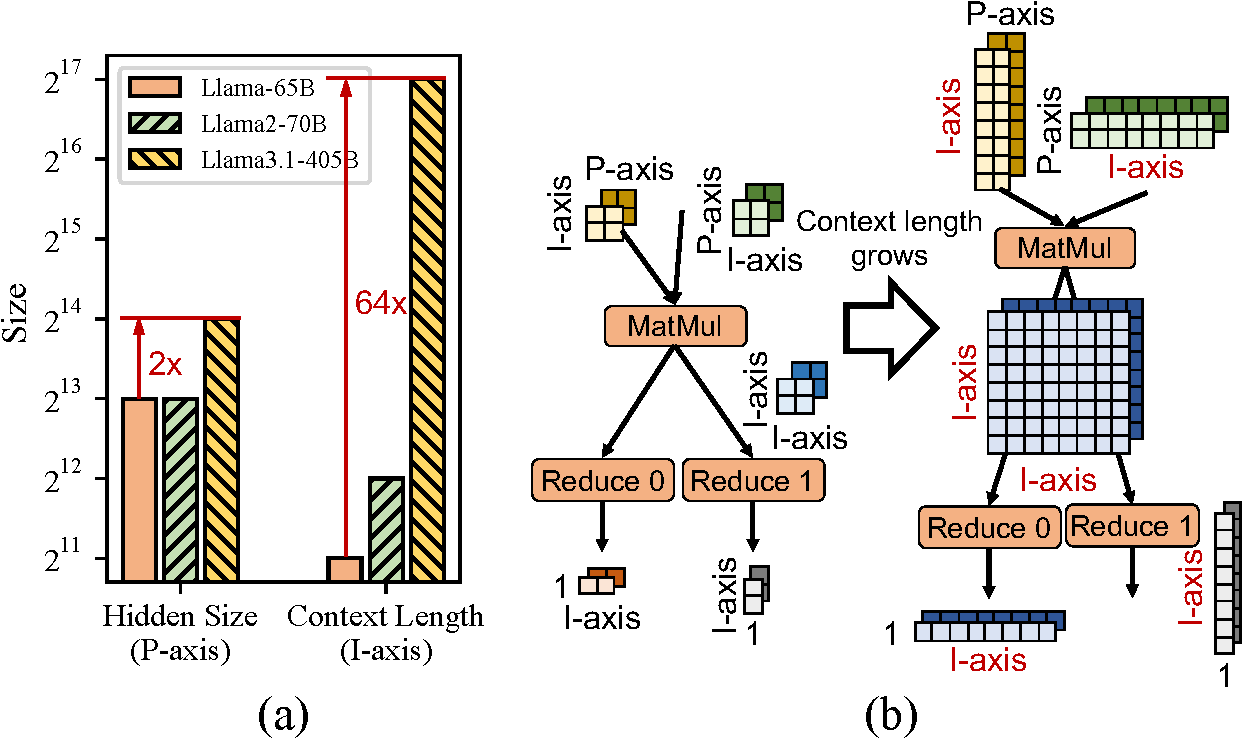
\includegraphics[width=0.85\linewidth]{figures/flashtensor/intro_workload-crop.pdf}
    % \vspace{-2em}
    \caption{模型张量增长情况与注意力变体示例}
    % \vspace{-1.5em}
    \label{fig:flashtensor-larger_workload}
\end{figure}

经调研总结,本文发现这两个方面的增长速度存在明显差异。
例如,从 Llama-65B 到 Llama-3.1-405B~\cite{touvron2023llama, touvron2023llama2, dubey2024llama3},P维度(隐藏层大小)从 8k 增加到 16k,仅增长了 2 倍;
而 I 维度(上下文长度)从 2k 扩展到 128k,增长了 64 倍,如\Cref{fig:flashtensor-larger_workload}(a)所示。
不同轴的增长速度差异导致模型中间张量的大小与形状出现显著变化。
\Cref{fig:flashtensor-larger_workload}(b)展示了注意力变体的一个简化部分计算图,其中包含一个矩阵乘法(MatMul)操作,
随后是两个不同归约方向的归约(Reduce)操作。
当 P 维度和 I 维度的大小相近时,MatMul 操作的输入和输出形状相似;
但在当前 P 维度和 I 维度大小差异巨大的情况下,MatMul 的输出相比计算中涉及的其他张量变得极其庞大。
这些巨大的张量需要耗费大量的处理时间,其计算效率对整体性能至关重要。

然而,由于算子操作的复杂性,当前的方法~\cite{tensorrt, torchcompile, zheng2023einnet, chen2018tvm, hu2024korch}在优化这些巨大张量时往往不能提供有效的解决方案。
如\Cref{fig:flashtensor-larger_workload}(b)所示,MatMul 的输出张量极大,融合是消除该张量并减少内存开销的有效方法之一。
但该张量随后被两个 Reduce 算子使用,一个按行归约,另一个按列归约。
如果进行融合,两个 Reduce 算子因不同归约维度导致的复杂依赖关系会降低并行性,大幅降低性能。
了解流经计算图边的中间张量的属性,如上述对特定轴的归约依赖,对于找到算子图的高效解决方案至关重要,更多有用的张量属性类型将在后文讨论。

在现有工作中,一方面,手动开发与优化算子库的研究~\cite{dao2022flashattention, dao2023flashattention, shah2024flashattention, ye2025flashinfer}虽然能够带来相对极致的性能,但无法涵盖层出不穷的众多新型模型结构变体。
另一方面,深度学习编译器~\cite{niu2021dnnfusion, astitch, shi2023welder}具备自动优化能力,但大多考虑张量大小、算子类型等相对粗粒度张量属性,往往忽略归约方向等细粒度张量属性,丢失了针对长序列场景下的深度优化机会。

本研究提出了 FlashTensor,通过利用细粒度张量属性来优化长序列后训练场景下的算子性能。
经研究观察,许多张量属性对于分析和优化以实现最佳性能至关重要,例如归约依赖、广播方向、大小和值等属性。
基于这一观察,FlashTensor 定义了张量的一些关键属性,并在计算图中识别它们,然后通过张量属性感知变换和内核映射策略优化张量程序。
本研究在 7 个模型上进行的实验,实验结果表明,与最先进的深度学习编译器相比,FlashTensor 的端到端加速比平均达到 1.50 倍,核心模块加速比平均达到 3.24 倍。
本章研究的主要贡献如下:

1. 总结了四个关键的细粒度张量属性,并设计了张量属性识别器,用于系统地分析整个计算图并捕获每个张量的属性。

2. 提出了细粒度张量属性感知的编译优化方法,基于属性感知变换规则和内核映射策略搜索最优内核,以实现高计算效率和低内存访问开销。

3. 基于上述设计实现了一个利用细粒度张量属性优化张量算子性能的系统 FlashTensor,其性能优于当前最先进的系统。

\begin{figure}[ht]
    \centering
    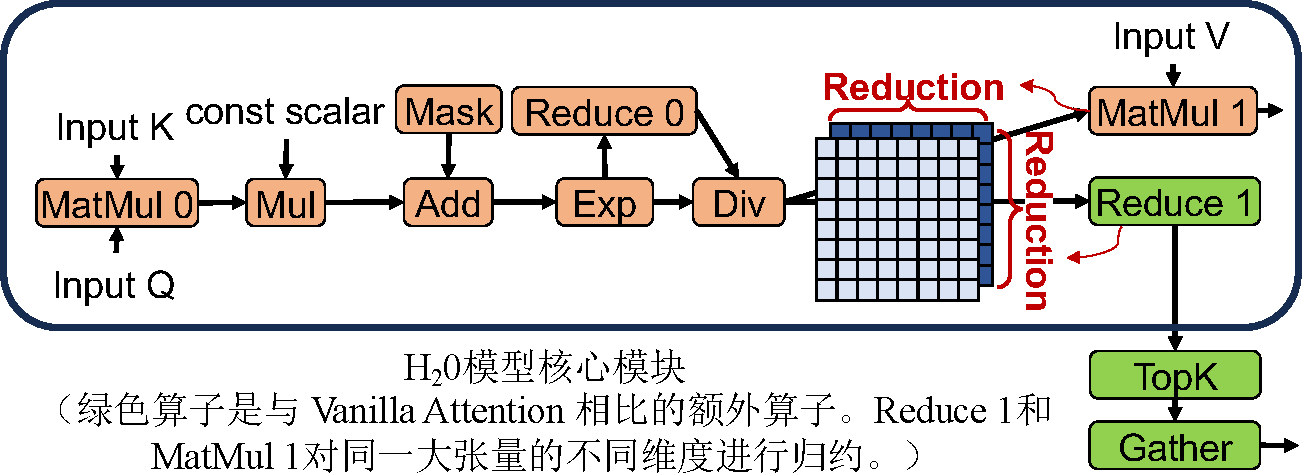
\includegraphics[width=0.7\linewidth]{figures/flashtensor/motivation_example_h2o_overview-crop.pdf}
    % \vspace{-1.7em}
    \caption{\(H_{2}O\) 模型示例}
    % \vspace{-2em}
    \label{fig:flashtensor-motivation_example_h2o_overview}
\end{figure}

\section{研究动机}

在大语言模型中,注意力机制是核心组件之一,负责捕捉输入序列中词元之间的依赖关系。
然而,传统的注意力机制在处理长上下文时会产生巨大的内存开销和计算量,尤其是在输入序列长度显著增加时。
在模型算法测,近期的一个研究热点是使用新的注意力变体来减少传统注意力机制的大量计算。
例如,\(H_{2}O\)~\cite{zhang2024h2o}、RoCo~\cite{ren2024roco} 和 Keyformer~\cite{adnan2024keyformer} 等模型可以丢弃一些不重要词元的数据以减少总计算量。
以\(H_{2}O\)为例(见\Cref{fig:flashtensor-motivation_example_h2o_overview}),它在 SoftMax(由 Exp、Reduce 0 和 Div 组成)之后使用一个额外的 Reduce 算子(Reduce 1)来计算词元的重要性,然后通过 TopK 算子结合 Gather 算子,选择并缓存最重要的词元数据,同时丢弃其余词元数据。

\(H_{2}O\)在后训练的推理过程时,包括两个阶段:预填充阶段(Prefill)和解码阶段(Decode)。
在预填充阶段,输入提示会被逐块处理,重要的词元会被选择并缓存数据,特别是当输入超过缓存容量时;
在解码阶段,输出词元数据会依次生成,并且在选择和保留最重要的词元数据时,缓存会进一步更新。
因此,新增的算子会影响预填充阶段和解码阶段的性能。
然而,对于长上下文文档摘要等任务,预填充阶段成为显著的性能瓶颈。
例如,在 InfiniteBench~\cite{zhang2024infinitebench} 中,提示的词元数可达 442K,而生成的词元数仅为 0.7K,相差 631 倍,导致\(H_{2}O\)中预填充与解码的执行时间比达到 4.51。
主要瓶颈源于预填充阶段核心模块中创建的大张量(见\Cref{fig:flashtensor-motivation_example_h2o_overview}),该张量由 MatMul 0 产生,大小为\(O(seqlen ^{2})\),导致大量的内存访问开销。
即使经过 TensorRT~\cite{tensorrt} 优化,\(H_{2}O\)的核心模块仍约占预填充总时间的 57.62\%,但计算性能仅达到 10.77 TFLOP/s(仅为 A100 F16 TensorCore 峰值性能的 3.45\%)。

关键挑战在于 MatMul 1 和 Reduce 1 这两个归约操作,它们对 Div 的输出张量(DivOut)具有不同的归约维度。为了提高效率,DivOut 的每一行必须分配到相同的并行单元用于 MatMul 1 操作,每一列也必须位于单个并行单元内。因此,除了使用单个并行单元外,没有其他可行的 DivOut 分区策略能满足这些约束。结果,像 TensorRT 这样的现有方法必须通过缓慢的全局内存跨多个内核处理大张量。此外,这两个具有不同归约维度的归约算子是\(H_{2}O\)与传统注意力机制的主要区别,由于这些结构差异,FlashAttention~\cite{dao2023flashattention} 难以对\(H_{2}O\)进行优化,其局限性源于缺乏对细粒度张量属性(如每个维度的归约依赖)的感知,从而错失了将 MatMul 1 与之前算子融合以避免访问大张量的机会。

\section{系统概述}

本研究通过利用细粒度张量属性来发掘更多算子融合机会,从而减少内存开销,提升推理运算性能。本节首先阐述对关键张量属性的观察,然后介绍FlashTensor系统设计。

\subsection{观察}

本小节列出一些细粒度的张量属性,并以\(H_{2}O\)模型为例说明它们为何对于发掘更多算子融合机会很重要。

\begin{itemize}

\item 
\textbf{归约依赖}:归约依赖指的是张量的某些维度是否会被聚合或归约,这对于分析算子的潜在并行机会至关重要。
如前所述,在\Cref{fig:flashtensor-motivation_example_h2o_overview}中,Div 的输出张量存在两个方向的归约依赖。
Reduce 1 无法在行维度上进行跨流式多处理器(SM)并行化,MatMul 1 无法在列维度上并行化,这使得整个计算图难以并行化。
识别这种归约依赖对于避免次优的并行化模式并寻找最优策略至关重要。
\item
\textbf{广播}:广播是指张量的维度被扩展或广播以匹配另一个张量的形状。
例如,\Cref{fig:dependency_and_broadcast_example}中的 Mul 算子隐式地对其右侧操作数的列维度进行广播。
何时进行广播对总计算量很敏感,图中示例里,重新排序后乘法计算量从\(NNh\)减少到\(Ndh\)。
但这种重新排序并不总是能得到正确结果,验证此类变换需要深入分析归约轴和广播轴之间的关系,这将后文进一步讨论。
\item
\textbf{大小}:大小是张量的固有属性,表示其包含的元素总数,与内存访问量密切相关,减少内存访问开销的关键策略之一就是最小化张量大小。
\item
\textbf{值}:值属性有助于减少不必要的计算和内存访问。例如,当了解到解码器-Transformer 中常用的三角掩码以及其上算子的含义后,可以跳过大多数张量中一半的计算。

\end{itemize}

\begin{figure}[htbp]
    \centering
    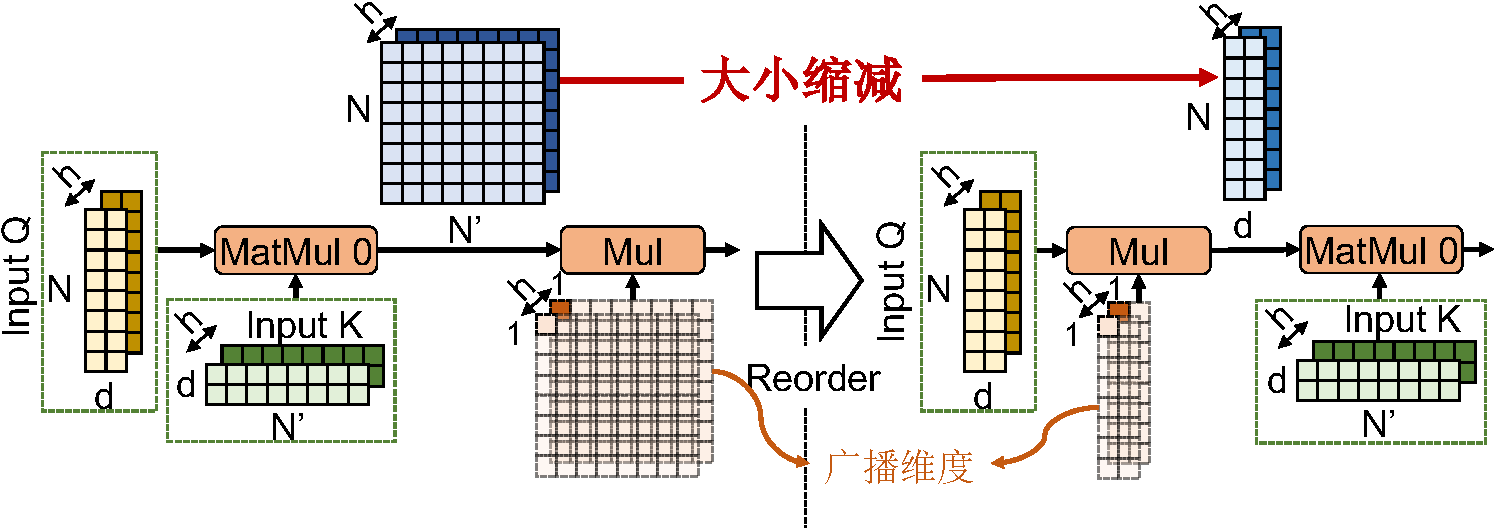
\includegraphics[width=0.7\linewidth]{figures/flashtensor/motivation_example_dependency_and_value-crop.pdf}
    % \vspace{-2em}
    \caption{\(H_{2}O\)模型中的广播示例}
    % \vspace{-1.7em}
    \label{fig:dependency_and_broadcast_example}
\end{figure}

\subsection{FlashTensor 系统设计}
基于上述观察,本研究提出了考虑这些细粒度张量属性的 FlashTensor。
如研究动机部分所述,FlashTensor 专注于优化长上下文任务的瓶颈——预填充阶段。
\Cref{fig:flashtensor-overview}展示了 FlashTensor 的总体架构,它主要由两个模块组成:张量属性识别器和张量属性感知优化器。
首先,张量属性识别器模块将张量程序作为输入(以计算图表示,节点表示算子,边表示张量),并捕获计算图中每个张量的所有细粒度属性,包括归约依赖、广播、大小和值。
然后,张量属性感知优化器模块根据图变换规则和内核映射策略搜索最优方案。
图变换规则旨在在特定限制下减小中间张量的大小,内核映射策略则通过考虑内存访问、计算强度和并行性来寻找高效的候选内核。
最终生成优化后的张量程序,可作为高效代码执行。

\begin{figure}[ht]
    \centering
    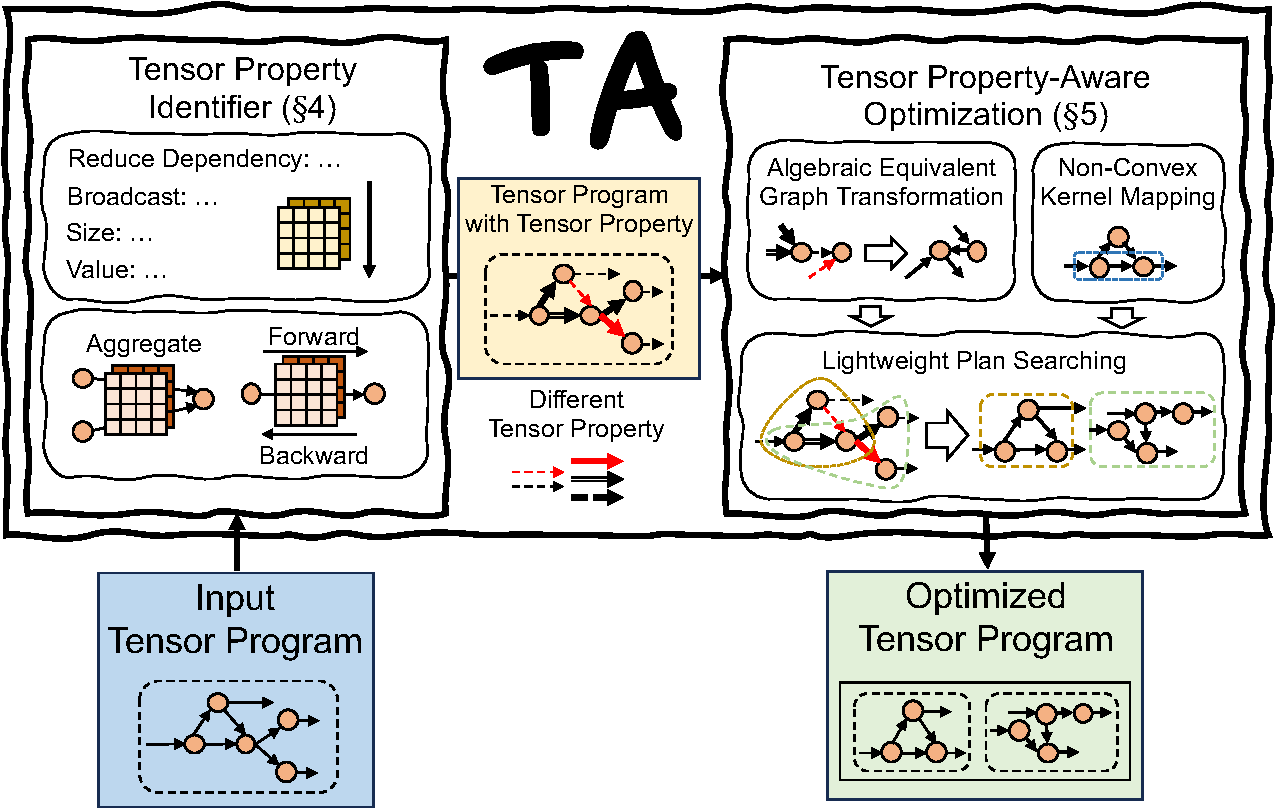
\includegraphics[width=0.7\linewidth]{figures/flashtensor/overview-crop.pdf}
    % \vspace{-1.5em}
    \caption{FlashTensor系统设计}
    % \vspace{-2em}
    \label{fig:flashtensor-overview}
\end{figure}



\section{张量属性识别器}
本节首先正式定义对后续分析和优化至关重要的张量属性,然后介绍 FlashTensor 如何在计算图中识别这些属性。



\subsection{属性定义}
如\Cref{tab:property}所示,张量属性分为两个不同类别:
1){逐维属性}:张量单个维度的特定属性,提供有关归约依赖和广播能力等方面的信息;
2){整体张量属性}:涵盖描述整个张量的属性,如总大小和可能的常数值。

\begin{table}[ht]
\centering
% \footnotesize
\caption{FlashTensor中的张量属性}
% \vspace{-0.5em}
\begin{tabular}{p{1.4cm}<{\centering}cp{4.2cm}}
\toprule
\multicolumn{3}{c}{\textbf{逐维度属性}} \\

\hline
\multirow{3}{*}{\makecell{归约\\依赖}} & \multirow{1}{*}{\makecell{NonPara}} & 不可并行化维度 \\
                             & \multirow{1}{*}{\makecell{Batch}} & 完全可并行化维度 \\
                             & \multirow{1}{*}{\makecell{Reuse}} & 具有数据复用的可并行化维度 \\
\hline

\multirow{2}{*}{\makecell{广播}} & No & 未广播维度 \\
                           & Yes & 已广播维度 \\
\hline
\multicolumn{3}{c}{\textbf{整体张量属性}} \\
\hline
\makecell{大小} & 整数 & 张量的总大小 \\
\hline
\multirow{7}{*}{\makecell{值}} & Var & 张量值未确定 \\
                       & Zero & 全零张量 \\
                       & PosConst & 正常量张量 \\
                       & NegConst & 负常量张量 \\
                       & PosInf & 正无穷大张量 \\
                       & NegInf & 负无穷大张量 \\
                       & NaN & 非数值张量 \\
\bottomrule
\end{tabular}
% \vspace{-1.0em}
\label{tab:property}
\end{table}


\begin{itemize}
\item
\textbf{归约依赖}:归约依赖属性是一个多值属性,描述张量维度与归约操作之间的相互依赖关系,这对优化计算效率至关重要。
它有三个取值:
1) NonPara:表示由于归约操作的数据依赖,无法进行并行执行分区的维度。这些维度需要由单个单元处理,无法并行化。例如,在\Cref{fig:property_definition_dependency}(a)中,输入和输出的归约维度都被归类为 NonPara,因为它们需要在整个维度上进行数据聚合。
2) Reuse:表示可以并行化且能通过分块实现数据重用的维度。例如,在\Cref{fig:property_definition_dependency}(b)中,MatMul 的行维度可以并行化,通过分块重用右侧操作数可提高内存效率,这种方法也适用于支持广播的操作,如 Add 和 Mul,分块后并行化可平衡计算效率和内存访问。
3) Batch:表示可以完全并行化且无需数据重用的维度,如\Cref{fig:property_definition_dependency}(b)中批量矩阵乘法的批次维度,以及\Cref{fig:property_definition_dependency}(a)中 Reduce 操作除归约维度外的其他维度。

\begin{figure}[ht]
    \centering
    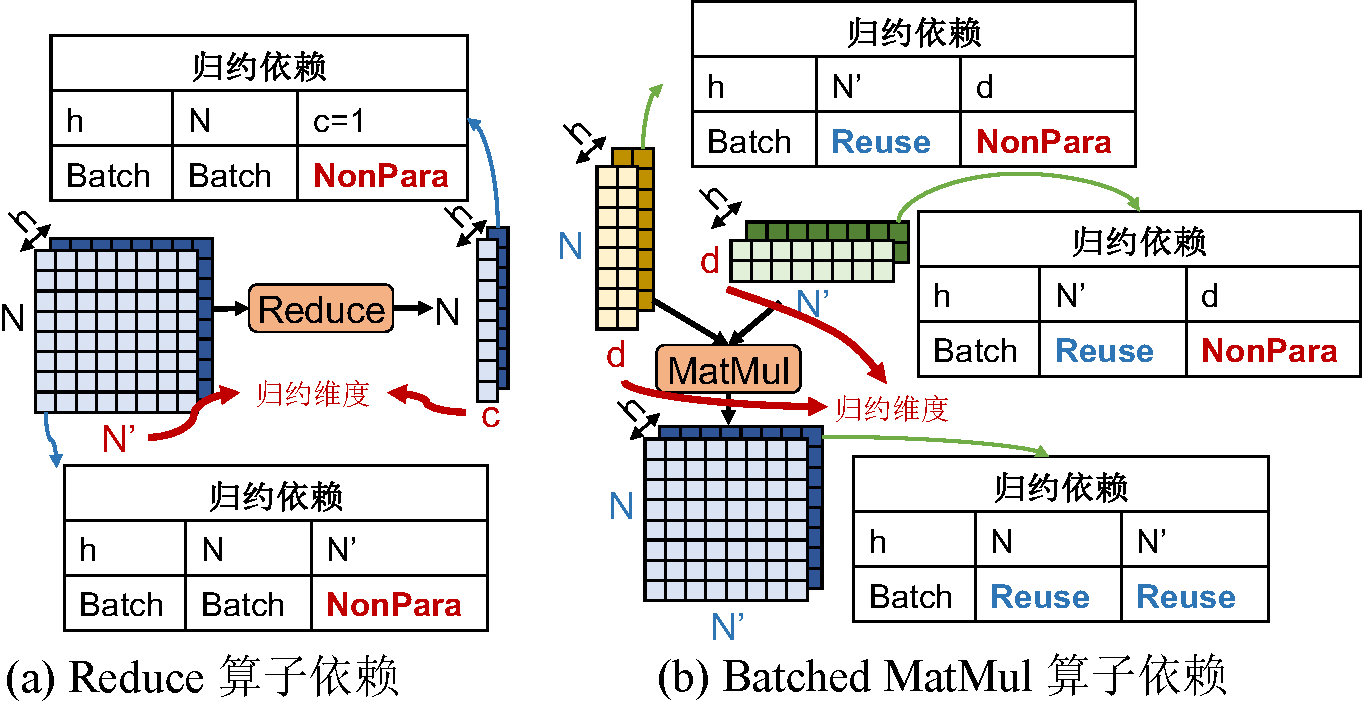
\includegraphics[width=0.7\linewidth]{figures/flashtensor/property_definition_dependency-crop.pdf}
    % \vspace{-1.9em}
    \caption{归约依赖属性}
    % \vspace{-1.5em}
    \label{fig:property_definition_dependency}
\end{figure}

\item
\textbf{广播}:该属性表示张量的某个维度是否会被后续算子广播。如果张量在某维度上是支持广播算子的操作数,则该维度被视为广播维度。\Cref{fig:property_definition_broadcast}(a)(b)展示了维度如何扩展以满足算子形状要求的示例。
\item
\begin{figure}[ht]
    \centering
    % \includegraphics[width=0.93\linewidth]{figures/property_definition_broadcast-crop.pdf}
    \includegraphics[width=0.65\linewidth]{figures/flashtensor/property_definition_broadcast-crop.pdf}
    % \vspace{-1em}
    \caption{广播属性}
    % \vspace{-1.5em}
    \label{fig:property_definition_broadcast}
\end{figure}

\textbf{大小}:表示张量中元素的总数,计算为所有维度的乘积,如\Cref{fig:property_definition_size_and_value}所示。
\item
\textbf{值}:指示张量在计算过程中是否保持常数值,如\Cref{fig:property_definition_size_and_value}所示。
与传统编译器将常量视为标量不同,FlashTensor 在张量级别处理常量,从而提供更广泛的优化机会。
具有常数值的张量可以预先计算或高效存储,减少执行期间的动态更新。
在 FlashTensor 中,常数值信息以枚举形式表示,而非实际值,以平衡信息有效性和开销。
\end{itemize}





\begin{figure}[htbp]
    \centering
    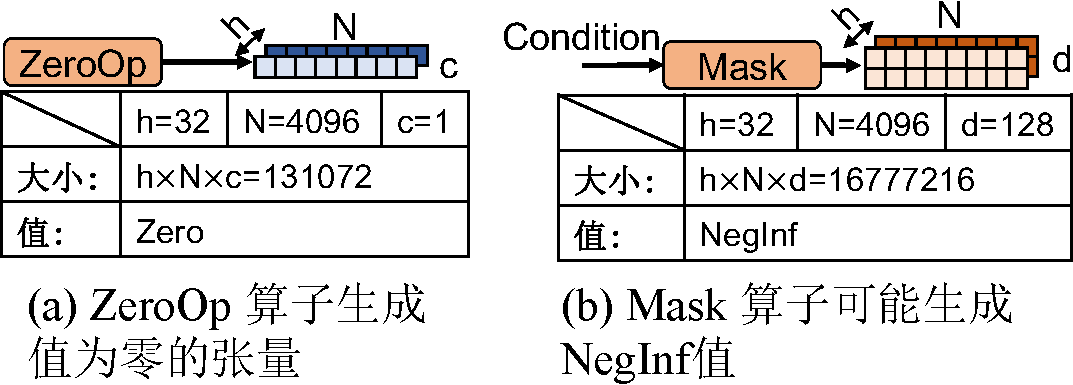
\includegraphics[width=0.52\linewidth]{figures/flashtensor/property_definition_size_and_value-crop.pdf}
    % \vspace{-0.7em}
    \caption{大小和值属性}
    % \vspace{-2em}
    \label{fig:property_definition_size_and_value}
\end{figure}



% \begin{table}[h]
% \footnotesize
% \caption{Tensor properties in FlashTensor. The second column lists the potential values for each corresponding property.}
% % \vspace{-0.5em}
% \begin{tabular}{|p{1.4cm}<{\centering}|c|p{4.2cm}|}
% \hline
% \multicolumn{3}{|l|}{\textbf{Per-Dimension Property}} \\

% \hline
% \multirow{3}{*}{\makecell{Reduce\\dependency}} & \multirow{1}{*}{\makecell{NonPara}} & Non-parallelizable dim. \\
%                              & \multirow{1}{*}{\makecell{Batch}} & Embarrassingly parallelizable dim. \\
%                              & \multirow{1}{*}{\makecell{Reuse}} & Parallelizable dim with data reuse. \\
% \hline

% \multirow{2}{*}{\makecell{Broadcast}} & No & Unbroadcasted dim. \\
%                            & Yes & Broadcasted dim. \\
% \hline
% \multicolumn{3}{|l|}{\textbf{Entire Tensor Property}} \\
% \hline
% \makecell{Size} & An integer & The total size of the tensor. \\
% \hline
% \multirow{7}{*}{\makecell{Value}} & Var & The tensor value is undetermined. \\
%                        & Zero & The tensor is all zero. \\
%                        & PosConst & The tensor is a positive constant. \\
%                        & NegConst & The tensor is a negative constant. \\
%                        & PosInf & The tensor is positive infinity. \\
%                        & NegInf & The tensor is negative infinity. \\
%                        & NaN & The tensor is not a number. \\
% \hline
% \end{tabular}
% % \vspace{-1.0em}
% \label{tab:property}
% \end{table}

\subsection{基于数据流的属性识别}
一些基本属性(如大小)可以很容易地从张量中提取,但像归约依赖这样的复杂属性则需要复杂的分析才能准确标注。
例如,在单个算子中,即使不完全实现算子,也可以根据其计算语义简单标注输入和输出张量的归约依赖,如\Cref{fig:property_definition_dependency}所示。
然而,在包含多个算子的计算图中,张量的归约依赖属性会受到后续和前面算子的影响,难以确定其确切值。

为解决这个问题,本研究提出了一种基于两阶段数据流的属性识别算法:
1) \textbf{属性传播}:根据每个算子的计算语义,张量属性进行前向和后向传播。
2) \textbf{属性聚合}:将从各个算子传播来的属性进行聚合,以确定每个张量的最终属性值。
该算法利用固有的单调优先级(例如,归约依赖类型:NonPara > Reuse > Batch)。
当不同类型的属性在同一张量维度上汇聚时,保留优先级较高的值,以确保在整个图中准确表示属性。
这些阶段会迭代执行,直到属性稳定。
\Cref{fig:identification_merge}给出了归约依赖识别的示例以进一步说明。\Cref{fig:identification_merge}(b)展示了 MatMul 的输出如何通过后向传播将右侧操作数在 N’维度上的归约依赖从 Reuse 更新为 NonPara;\Cref{fig:identification_merge}(a)展示了 MatMul 和 Reduce 之间的属性聚合过程,中间张量从两个算子接收不同的归约依赖值。

\begin{figure}[ht]
    \centering
    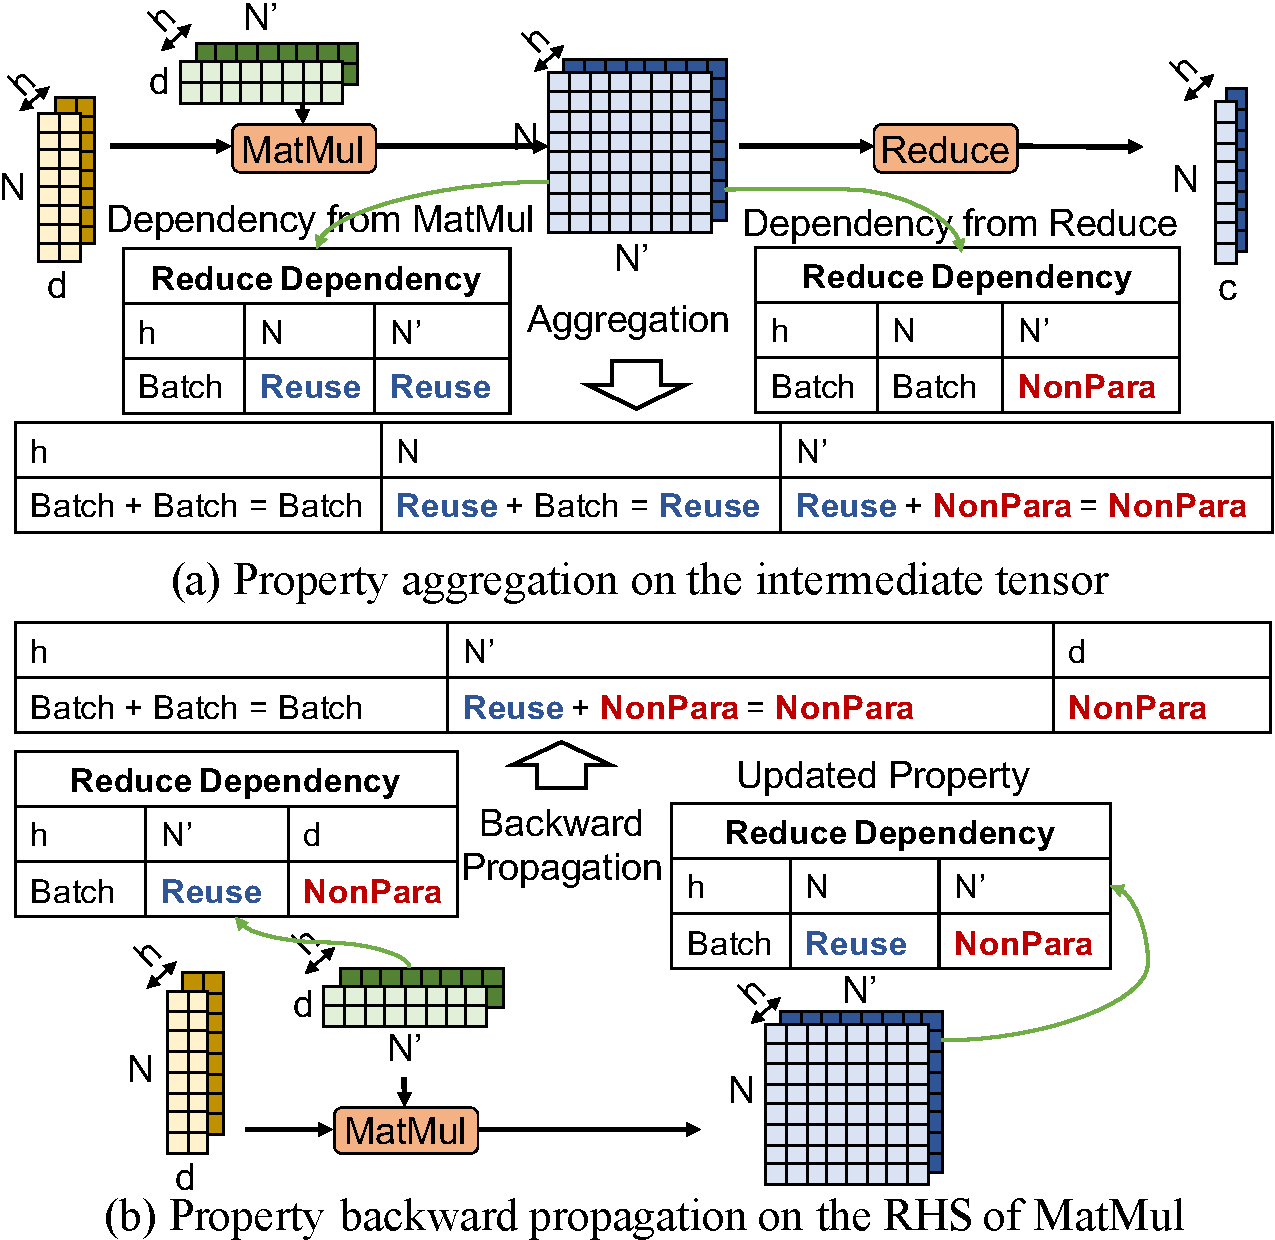
\includegraphics[width=0.7\linewidth]{figures/flashtensor/identification_merge-crop.pdf}
    % \vspace{-1.5em}
    \caption{归约依赖属性识别示例}
    % \vspace{-1em}
    \label{fig:identification_merge}
\end{figure}

\section{细粒度张量属性感知优化}
FlashTensor 基于识别出的细粒度张量属性进一步优化张量程序。
优化基于两个规则(代数等价图变换和非凸内核映射)以及一种轻量级方案搜索方法。
代数等价图变换提供一系列变换规则,允许通过等价变换改变中间张量的大小;
非凸内核映射提出一种新的候选内核以实现高效执行;
轻量级方案搜索通过属性约束剪枝和低成本性能模型实现高效的方案生成。

\subsection{代数等价图变换}
中间张量的大小是决定内存访问开销的主要因素。
因此,本研究提出一种变换方法,主要通过对计算图进行代数等价变换来关注中间张量大小的变化,这使得后续能够在整个搜索空间中寻找中间张量大小最小的计算图,从而减少内存开销。
{广播是导致中间张量大小变化的本质原因}。


\begin{table}[ht]
    \centering
    \caption{基于广播属性的转换规则}
    % \vspace{-0.5em}
    % \footnotesize
    \begin{tabular}{ccc}
       \toprule
       规则  & 注释 & 条件 \\
       \hline
       $A + B = B + A$  & 交换律 & 否 \\  
       $A \odot B = B \odot A$  & 交换律 & 否 \\  
       
       $A + (B + C) = (A + B) + C$  & 结合律 & 否 \\  
       $A \odot (B \odot C) = (A \odot B) \odot C$  & 结合律 & 否 \\  
       $\sum_i(A + B) = \sum_iA + \sum_iB$ & 结合律 & 否 \\

       $A \odot C + B \odot C = (A + B) \odot C$ & 分配律 & 否 \\
       $A / C + B / C = (A + B) / C$ & 分配律 & 否 \\

        \hline

       $\sum_i(A \odot B) = (\sum_iA) \odot (\sum_iB)$ & 分配律 & 是 \\
       \multicolumn{3}{r}{若 $A \odot B$ 中 $A$ 或 $B$ 在维度 $i$ 上被广播} \\
       
       $\sum_i(A / B) = (\sum_iA) / (\sum_iB)$ & 分配律 & 是 \\
       \multicolumn{3}{r}{若 $A / B$ 中 $B$ 在维度 $i$ 上被广播} \\
       
       $(A \odot B)C = (AC) \odot B$ & 分配律 & 是 \\
       \multicolumn{3}{r}{若 $B$ 在 $AC$ 的归约维度上被广播} \\
       
       $(A / B)C = (AC) / B$ & 分配律 & 是 \\
       \multicolumn{3}{r}{若 $B$ 在 $AC$ 的归约维度上被广播} \\
       \bottomrule
    \end{tabular}
    % \vspace{-1.5em}
    \label{tab:broadcast_based_transform}
\end{table}




(1) \textbf{基于广播属性的变换规则}:本研究提出了一系列变换规则,这些规则不仅考虑张量大小,还考虑每个维度的广播属性。具体而言,\Cref{tab:broadcast_based_transform}列出了所有变换规则。$A$、$B$ 和 $C$ 为张量。$+$、$\odot$ 和 $/$ 分别为逐元素加、乘和除。$AB$ 表示 $A$ 和 $B$ 的矩阵乘法。除矩阵乘法外的所有运算符均支持广播。主要规则可分为两大部分:
始终有效的变换:无论操作数的广播属性如何,这些变换始终有效,其有效性由不同算子及其组合的交换律、结合律和分配律这三个数学定律保证。

\begin{figure}[ht]
    \centering
    % \includegraphics[width=0.8\linewidth]{figures/wo_broadcast-crop.pdf}
    \includegraphics[width=0.75\linewidth]{figures/flashtensor/wo_broadcast-crop.pdf}
    % \vspace{-0.7em}
    \caption{MatMul 与 Div 算子重排序示例}
    % \vspace{-1.3em}
    \label{fig:wo_broadcast}
\end{figure}

(2) \textbf{受广播属性约束的变换}:某些变换的有效性取决于广播属性。在这些变换中,广播被视为确保正确性的关键属性。例如,在\Cref{fig:wo_broadcast}(a)中,当 Div 的右侧操作数在 N 维度上广播时,重新排序是无效的,因为 MatMul 中的归约会破坏计算语义,导致结果错误;而在\Cref{fig:wo_broadcast}(b)中,如果 Div 的右侧操作数沿与 MatMul 归约维度对齐的维度广播,重新排序则是有效的。

(3) \textbf{基于值属性的变换规则}:本研究利用值属性通过消除不必要的迭代来优化循环。具体而言,重点是在不影响最终输出的情况下跳过 For 循环中的某些迭代。如\Cref{fig:value_example}所示,某些迭代可能会从 Mask 算子产生常量值(如 -∞),由于这些常量值在 For 循环中保持不变地传播,FlashTensor可以识别并安全地跳过这些迭代,这不仅保持了输出的正确性,还减少了计算量。

\begin{figure}[ht]
    \centering
    % \vspace{-1em}
    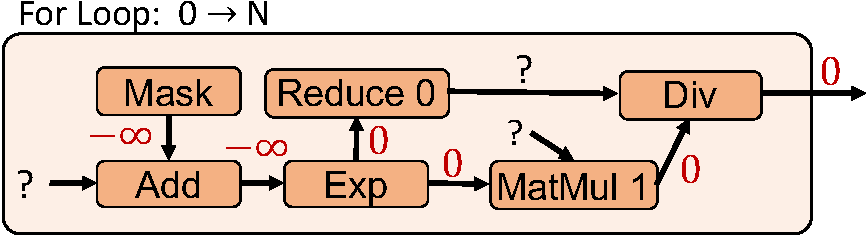
\includegraphics[width=0.5\linewidth]{figures/flashtensor/value_example-crop.pdf}
    % \vspace{-1em}
    \caption{值属性示例}
    % \vspace{-1em}
    \label{fig:value_example}
\end{figure}


\subsection{非凸内核映射}
内核映射是指在现代硬件平台上将计算图中的算子分配给 GPU 内核执行。
对于给定的计算图,简单地将所有算子融合到单个内核中,由于复杂的归约依赖和有限的并行性,往往会导致性能不佳,因此识别合适的内核以实现高效执行至关重要。

首先,本文给出最先进研究中内核的形式化定义。

\vspace{0.5em}
\begin{definition}[内核] 对于计算图\(G=(V, E)\),如果不存在节点\(p_{1}, p_{2} \in K\)和另一个节点\(q \in V/K\),使得\(p_{1} \stackrel{G}{\rightsquigarrow } q\)且\(q \stackrel{G}{\rightsquigarrow} p_{2}\)(其中\(x \stackrel{G}{\rightsquigarrow} y\)表示在\(G\)中存在从\(x\)到\(y\)的路径),则节点集\(K \subseteq V\)构成一个内核。
\end{definition}
\vspace{0.5em}

该定义将计算图中的凸子集算子视为内核,凸性意味着这种内核不能包含通过外部算子依赖自身的算子,如\Cref{fig:kernel_def_diff}(a)所示。
Korch~\cite{hu2024korch} 认为由于循环依赖(即 Div 依赖于 Reduce,Reduce 又依赖于 Exp),这样的内核无法执行,但这种循环依赖可以通过其他内核解决,具体而言,一个内核不必生成自身输入,只要有其他内核提供这些输入即可。
例如,为解决\Cref{fig:kernel_def_diff}(a)中的循环依赖,包含 Exp 和 Reduce 的另一个内核可以提供输入,从而使包含 Div 的内核能够顺利执行。基于这一理解,本研究放宽了传统内核定义的限制,提出了非凸内核的概念。

\vspace{0.5em}
\begin{definition}[非凸内核] 对于计算图\(G=(V, E)\),当且仅当存在一个存在节点\(p_{1}, p_{2} \in K\)和另一个节点\(q \in V/K\),使得\(p_{1} \stackrel{G}{\rightsquigarrow } q\)且\(q \stackrel{G}{\rightsquigarrow} p_{2}\),节点集\(K \subseteq V\)构成一个非凸内核。
\end{definition}
\vspace{0.5em}

非凸内核的引入为算子的分配提供了更大的灵活性,有助于更好地适应复杂的计算图结构。
在确定内核时,本研究考虑了计算强度、内存访问模式和并行性等因素。
计算强度较高的算子倾向于被组合在一起,以充分利用硬件的计算资源。
同时,尽量减少内核之间的数据传输,以降低内存访问开销。
例如,对于具有相似内存访问模式的算子,将它们映射到同一个内核中,可以减少内存访问的次数和延迟。

\begin{figure}[ht]
    \centering
    % 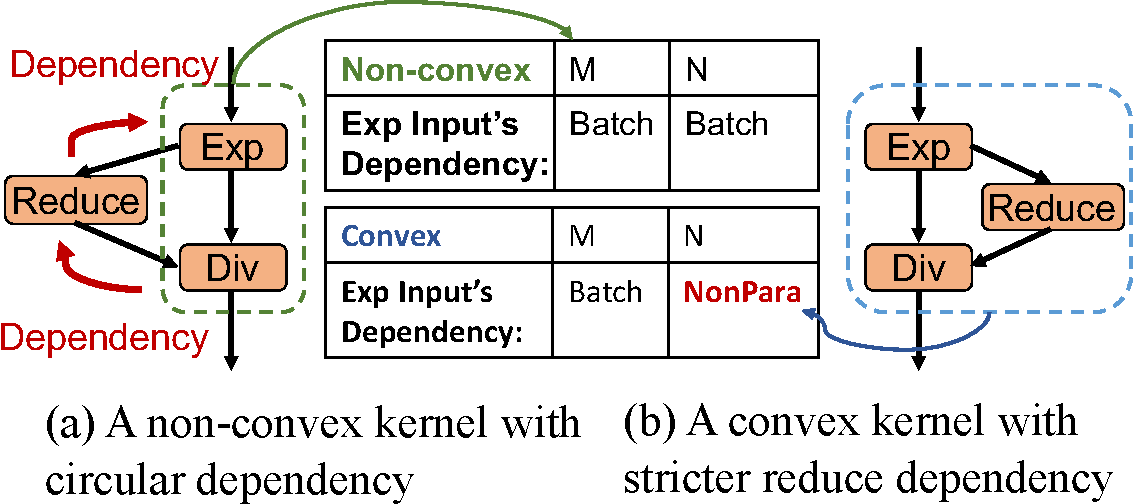
\includegraphics[width=0.85\linewidth]{figures/kernel_def_diff-crop.pdf}
    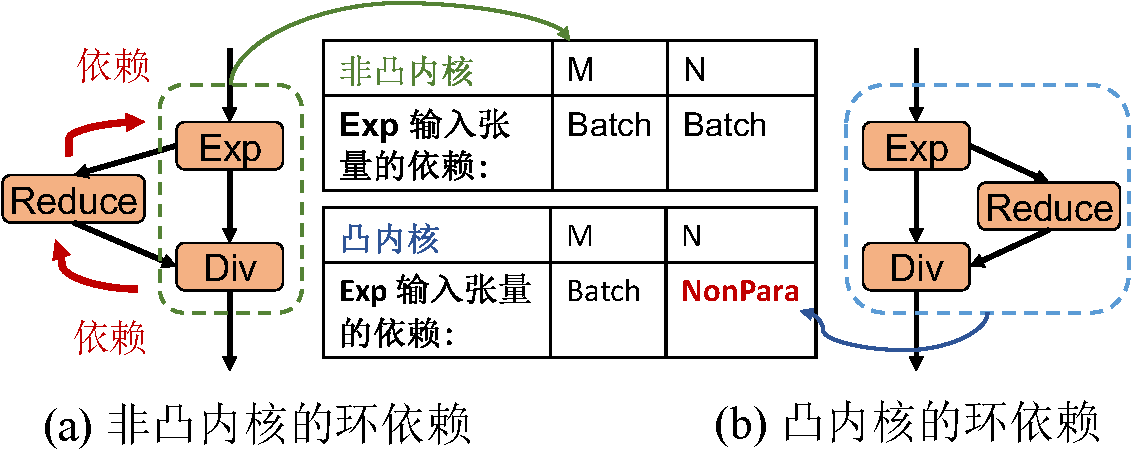
\includegraphics[width=0.6\linewidth]{figures/flashtensor/kernel_identification-crop.pdf}
    % \vspace{-0.8em}
    \caption{非凸内核与凸内核示例}
    % \vspace{-1.5em}
    \label{fig:kernel_def_diff}
\end{figure}


\subsection{轻量级方案搜索}
为了找到最优的内核映射方案,本研究采用了一种基于搜索的方法。该方法从一个初始的内核映射方案出发,通过对算子的分配进行小的调整,生成一系列候选方案。对于每个候选方案,本研究评估其性能,包括计算时间、内存使用量等指标。评估过程使用了一个轻量级的性能模型,该模型基于硬件的特性和算子的属性,能够快速估算出不同方案的性能表现。通过不断迭代搜索过程,逐步找到性能最优的内核映射方案。

在搜索最优的计算图变换和内核映射方案时,由于可能的方案数量庞大,穷举搜索是不可行的。因此,本研究提出了一种轻量级的方案搜索方法,该方法结合了属性约束剪枝和低成本性能模型,以高效地生成有潜力的方案。

(1) \textbf{属性约束剪枝}:本研究利用在张量属性识别阶段得到的张量属性信息,对搜索空间进行剪枝。
例如,如果一个张量的某个维度具有 NonPara 类型的归约依赖,那么在考虑并行化方案时,就可以排除那些涉及该维度并行化的方案,因为这些方案在实际执行中无法满足数据依赖要求,必然会导致性能不佳。
通过这种方式,能够显著减少需要评估的方案数量,提高搜索效率。

(2) \textbf{低成本性能模型}:为了快速评估不同方案的性能,本研究构建了一个低成本性能模型。
该模型考虑了算子的计算复杂度、内存访问开销以及硬件的特性。
例如,对于矩阵乘法算子,模型根据其输入矩阵的大小计算计算量;根据数据在内存中的存储布局和访问模式,估算内存访问时间。
通过将这些因素综合考虑,模型能够快速给出一个方案的性能估计值,允许在短时间内对大量候选方案进行评估和比较,从而筛选出有潜力的方案进行进一步优化。


整个搜索算法如\Cref {alg:kernel_identify}所示。
该算法首先确定可用的并行执行单元数量,例如 GPU SM的数量。
然后,遍历计算图的连通子集,筛选出并行度或算术强度低于性能阈值的内核。
在筛选出候选内核后,本研究遵循先前的工作~\cite{hu2024korch},将最优候选搜索形式化为一个二元线性规划任务并求解。

\begin{algorithm}[ht]
{
% \fontsize{8pt}{9pt}\selectfont
\caption{核识别}
    \label{alg:kernel_identify}
    % \small
    \SetAlgoNlRelativeSize{0}
    \SetAlgoNlRelativeSize{-1}
    \SetKwProg{Fn}{函数}{:}{}
    \KwData{计算图 $G$,算术强度阈值 $H$}
    \KwResult{$G$ 中的候选核 $K$}
    \Fn{搜索($G$)} { 
        $K = \emptyset $\; 
        最大并行单元数 $\leftarrow$ 查询底层加速器\;
        \ForEach{连通子集 $X$ $\in$ $G$}{
            $AI \leftarrow$ 计算 $X$ 的算术强度\;
            并行单元数 $\leftarrow$ 获取 $X$ 的并行度\;
            \If{$AI \geq H$ 且 并行单元数 $\geq$ 最大并行单元数}{
                $K = K \cup \{X\}$\;
            }
        }
        \Return $K$\;
    }
}
\end{algorithm}

\section{实验评估}
FlashTensor 基于 MLIR~\cite {lattner2020mlir} 和 Triton~\cite {tillet2019triton},由 10K 行 C++ 代码和 2K 行 Python 代码实现。
FlashTensor 以 ONNX 格式(可通过现有工具从原生 TensorFlow/PyTorch 程序轻松导出)为输入,并将其转换为有效的 MLIR 代码。
本研究在 MLIR 中实现了两种方言:FT 和 FTTriton。
FT 定义了张量操作(如逐元素操作、归约、重塑和矩阵乘法)以及通过 MLIR passes 实现的相应转换;
FTTriton 作为从 FT 到 Triton DSL 的桥梁,定义了与 Triton 类似的操作符。
应用所有优化后,最终的 MLIR 代码将转换为有效的 Triton 代码,接入PyTorch算子后端。

\subsection{实验设置}
实验平台方面,本研究在配备 NVIDIA A100 和 H100 GPU 的服务器上进行实验,以评估 FlashTensor 的性能。
具体为:
1)一块 NVIDIA A100-PCIE-40GB GPU(配备两颗 AMD EPYC 7742 64 核 CPU);
2)一块 H100-PCIE-80GB GPU(配备 AMD EPYC 7453 28 核 CPU)。
软件版本为 Python 3.10、CUDA 12.1 和 GCC 12.2。

评估模型方面,实验选取了七个具有代表性的模型,包括\(H_{2}O\)~\cite{zhang2024h2o}, RoCo~\cite{ren2024roco}, Keyformer~\cite{adnan2024keyformer}, SnapKV~\cite{li2024snapkv}, Corm~\cite{dai2024corm}, Vanilla Attention~\cite{vaswani2017attention} (V.A.), Gemma2~\cite{team2024gemma2}等新型注意力变体模型,以及一些传统基于 Transformer 的模型。
这些模型涵盖了不同的应用场景和计算特点,能够全面地测试 FlashTensor 的优化效果。
这些模型的简要描述如~\Cref {tab:model_description} 所示。
在端到端实验中,所有模型均使用  {Llama-2-7b}~\cite {touvron2023llama2} 作为基础模型,采用 FP16 精度权重、32 个注意力头和 128 的头维度。为保证公平比较,模型间唯一差异在于注意力模块设计。


\begin{table}[ht]
    \centering
    % \footnotesize
    \caption{评估模型的基本信息}
    % \vspace{-1em}
    \begin{tabular}{lp{12cm}}
       \toprule
       模型   & 描述 \\
       \hline
       \(H_{2}O\)   & 它利用累积注意力分数来丢弃对最终注意力分数贡献较小的高频词元。 \\
       % \hline
       RoCo   & 它注意到注意力概率的标准差与词元重要性之间的关系,并利用这种关系来指导词元丢弃。 \\
       % \hline
       Keyformer  & 它使用基于 Gumbel 软最大化的分数函数来识别关键词元。 \\
       % \hline
       SnapKV   & 它利用聚类来保留重要词元的注意力特征。 \\
       % \hline
       Corm   & 它定义了长期次要键,并丢弃被视为长期次要键的词元。 \\
       % \hline
       V.A.   & 它是当前基于Transformer的模型中广泛使用的标准注意力机制。 \\
       % \hline
       Gemma2   & 它是一种新提出的模型,为注意力层引入了对数软上限。 \\
       \bottomrule
    \end{tabular}
    % \vspace{-1.5em}
    \label{tab:model_description}
\end{table}

对比系统方面,本研究将 FlashTensor 与八种最先进的深度学习优化方法进行对比。
1) {深度学习编译器}: PyTorch 2.2.2~\cite{pytorch19} and corresponding TorchInductor~\cite{torchcompile}, TensorRT 10.0.1~\cite{tensorrt},  TVM 0.16.0~\cite{chen2018tvm} with MetaScheduler~\cite{chen2018autotvm, zheng2020ansor}, Korch~\cite{hu2024korch}, 以及 EinNet~\cite{zheng2023einnet}. 
2) {高效算子库}: FlashAttention 2.6.2~\cite{dao2022flashattention, dao2023flashattention} 以及 FlashInfer 0.1.0~\cite{ye2025flashinfer}.

在实验过程中,本研究统一使用相同的数据集对所有模型进行推理测试,以确保实验结果的可比性。
对于每个模型,本研究分别测量其端到端的推理时间以及核心模块的执行时间,并计算性能加速比。
同时,本研究还记录了内存使用情况,以评估 FlashTensor 在减少内存开销方面的效果。

% \begin{figure*}[ht]
%     \centering
%     \begin{minipage}[ht]{\textwidth}
%         {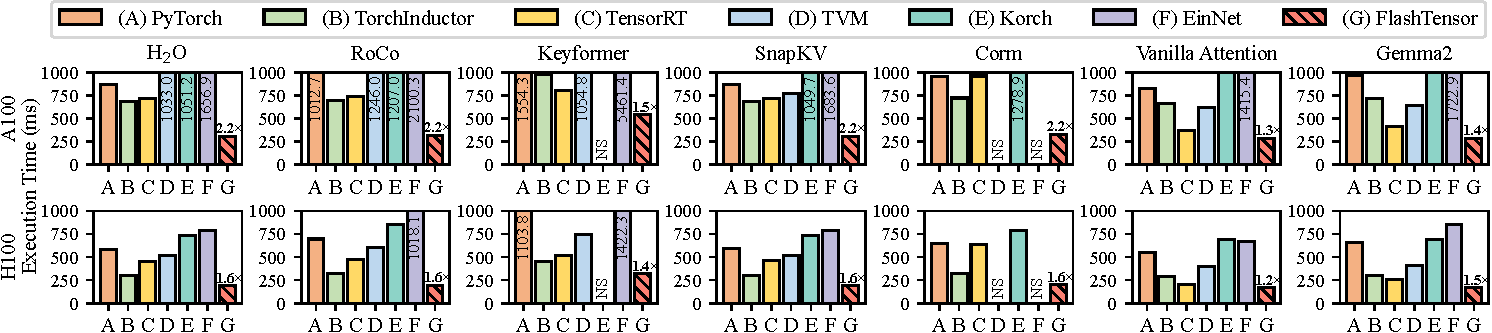
\includegraphics[width=\linewidth]{figures/flashtensor/e2e-crop.pdf}}
%         % \vspace{-1em}
%     \end{minipage}
%     \\
%     \centering \small (a) End-to-end performance
%     \begin{minipage}[ht]{\textwidth}
%         {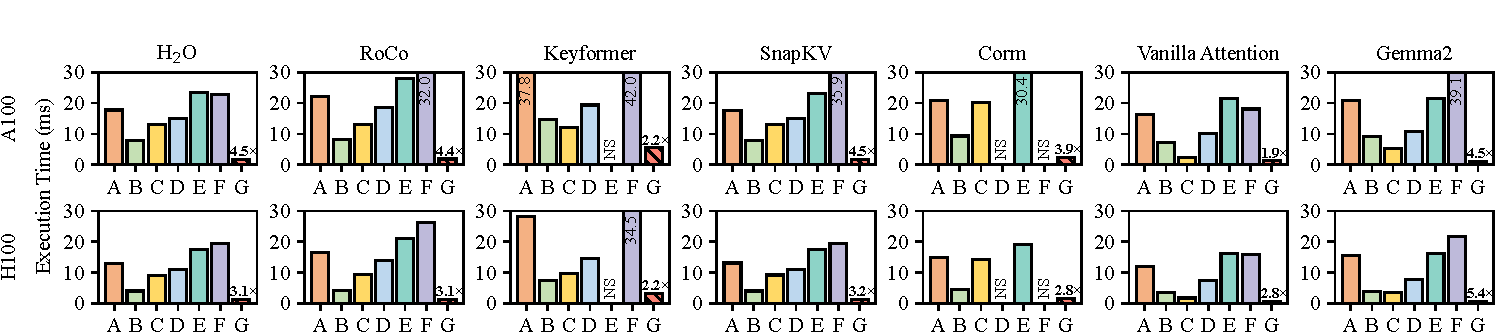
\includegraphics[width=\linewidth]{figures/flashtensor/kernel-crop.pdf}}
%         % \vspace{-1em}
%     \end{minipage}
%     \\
%     \centering \small (b) Core module performance
%     % \vspace{-1em}
%     \caption{End-to-end and core module performance comparison of seven evaluated models with SOTA systems on A100 and H100 GPU. NS means NotSupport. Bars for baselines of too long running time are truncated, and their execution times are marked on the bars. The numbers above FlashTensor's bars show FlashTensor's speedups over the best baseline.}
%     % \vspace{-0.5em}
%     \label{fig:e2e-kernel}
% \end{figure*}

\begin{figure}[ht]
    \centering
    \begin{minipage}[t]{\textwidth}
        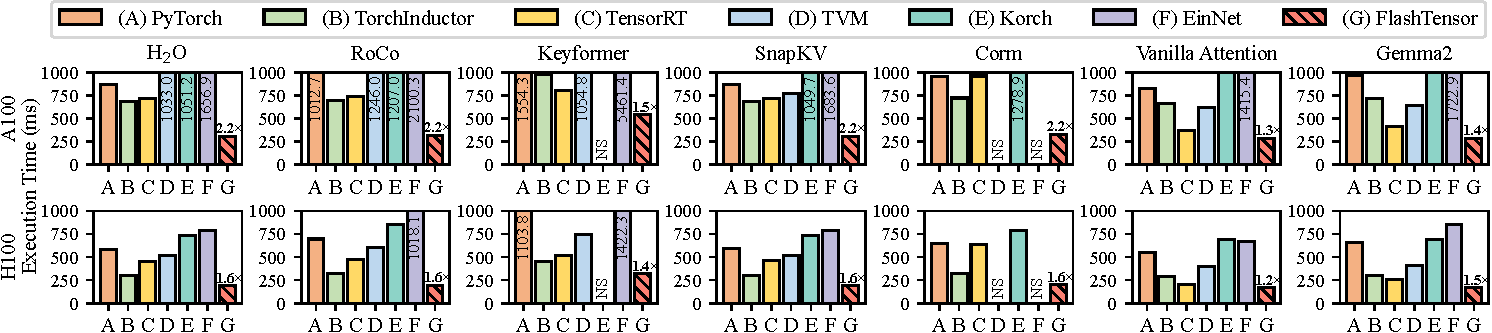
\includegraphics[width=\linewidth]{figures/flashtensor/e2e-crop.pdf}
    \end{minipage}
    \vspace{-0.5em}
    \caption*{\small (a) 端到端性能}
    
    \begin{minipage}[t]{\textwidth}
        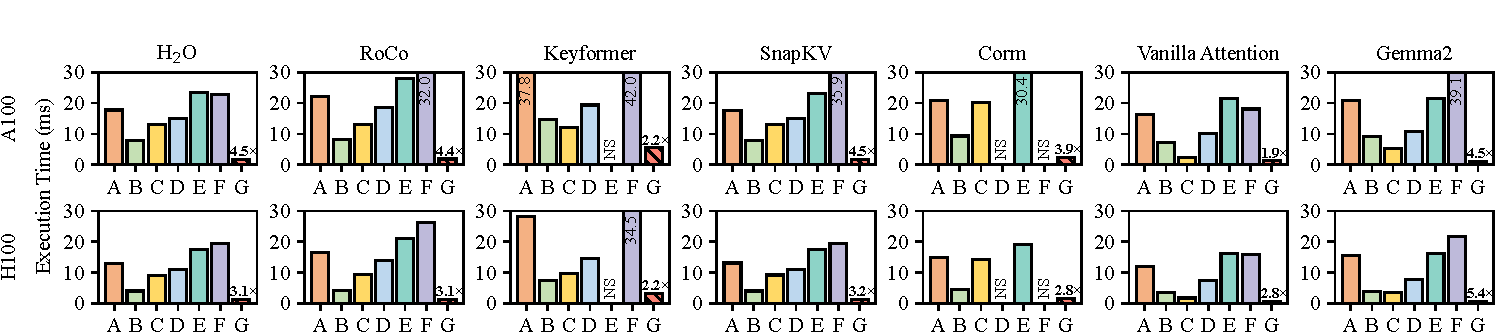
\includegraphics[width=\linewidth]{figures/flashtensor/kernel-crop.pdf}
    \end{minipage}
    \vspace{-0.5em}
    \caption*{\small (b) 核心模块性能}
    \caption{端到端和核心模块性能对比(A100和H100 GPU上)}
    \label{fig:e2e-kernel}
\end{figure}

\subsection{性能对比}

本研究首先比较了 FlashTensor 模型与最先进的深度学习编译器的端到端推理性能。
如\Cref {fig:e2e-kernel}所示,NS表示不支持,运行时间过长的基线柱状图被截断,其执行时间标注在柱状图上。
FlashTensor柱状图上方的数字显示了FlashTensor相对于最佳基线的加速比。

如\Cref {fig:e2e-kernel}(a) 所示,FlashTensor 在 A100 上的加速比最高可达最佳基线的\(2.22\times\),在 H100 上可达\(1.62\times\)。
FlashTensor 的性能提升主要来自高度优化的核心模块。
\Cref {fig:e2e-kernel}(b) 展示了核心模块(如注意力变体)的性能,FlashTensor 在 A100 上的加速比最高达\(4.52\times\),在 H100 上达\(5.43\times\)。

本研究观察到部分模型结构相似,在 FlashTensor 下性能大致相当,但经最先进的深度学习编译器优化后,性能差异显著。
例如,如~\Cref {fig:lib_cmp}(a) 所示,Gemma2 仅对标准注意力(V.A.)做了微小修改,绿色算子为 Gemma2 的额外结构。
使用 TensorRT 时,A100 上 Gemma2 和 V.A. 的推理时间分别为 5.13 和 2.25 毫秒——这种显著差距源于 TensorRT 针对 V.A. 的注意力结构预写了特定规则(类似 FlashAttention),但无法匹配 Gemma2 的微小修改结构。
而在 FlashTensor 中,A100 上 Gemma2 和 V.A. 的推理时间分别为 1.14 ms 和 1.20 ms,性能相当且超越 TensorRT。
这是因为 FlashTensor 通过张量属性感知规则自动搜索最优方案,既能适配不同模型,又能利用值感知循环迭代消除技术,进一步减少因果掩码导致的不必要计算。

\subsection{不同序列长度的可扩展性}
\Cref{fig:seqlen_mem_flops} 展示了 \(H_{2}O\) 在不同序列长度下的计算效率和内存占用可扩展性。  
\begin{figure}[ht]
    \centering
    % \vspace{-1.8em}
    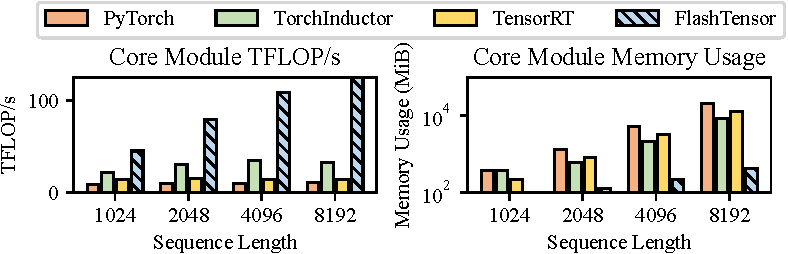
\includegraphics[width=0.7\linewidth]{figures/flashtensor/gflops_mem-crop.pdf}
    % \vspace{-1.7em}
    \caption{\(H_{2}O\) 在不同序列长度下的内存占用和 TFLOP/s}
    % \vspace{-0.5em}
    \label{fig:seqlen_mem_flops}
\end{figure}

计算效率方面,
每秒浮点运算次数(FLOP/s)是衡量内核计算效率或吞吐量的重要指标。
由于内存访问开销更低,FlashTensor 在序列长度较长时实现了更高的 FLOP/s。
TorchInductor 和 TensorRT 采用相同的内核映射策略,需在 CUDA 内核中从全局内存读写大小为 $O(\text{seqlen}^2)$ 的中间张量,从而导致高内存开销。  

内存占用方面,
本研究进一步通过内核的内存占用证明 FlashTensor 带来的中间张量尺寸缩减。
与 PyTorch 和 TensorRT 相比,FlashTensor 在全局内存中的内存占用显著更小,尤其是当序列长度增加时。
这种差异的主要原因在于 PyTorch 和 TensorRT 在慢速全局内存中分配与序列长度成二次方关系$O(\text{seqlen}^2)$的大中间张量,而 FlashTensor 旨在最小化此类大张量的分配,从而在序列长度增长时保持更高效稳定的内存使用。  

\begin{figure}[htbp]
    \centering
    \begin{minipage}[t]{\linewidth}
        \centering
        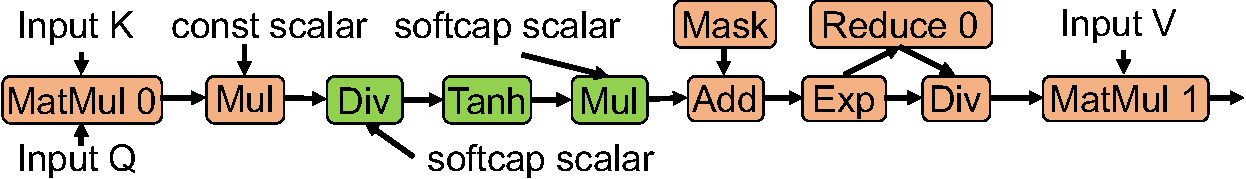
\includegraphics[width=0.75\linewidth]{figures/flashtensor/exp_gemma2-crop.pdf}
    \end{minipage}
    \vspace{-0.5em}
    \caption*{\small (a) 标准注意力与 Gemma2 的差异}
    
    \begin{minipage}[t]{\linewidth}
        \centering
        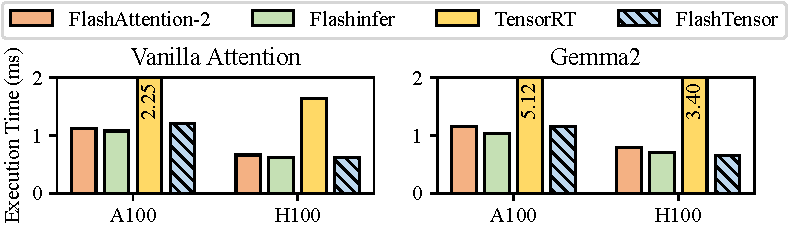
\includegraphics[width=0.7\linewidth]{figures/flashtensor/attn_time-crop.pdf}
    \end{minipage}
    \vspace{-0.5em}
    \caption*{\small (b) 标准注意力与 Gemma2 的执行时间}
    
    \caption{与算子库的对比}
    \label{fig:lib_cmp}
\end{figure}

\subsection{算子库对比实验}
本研究进一步将 FlashTensor 和 TensorRT 与手工调优的算子库 FlashAttention 和 FlashInfer 进行对比,这两个库均仅支持标准注意力(Vanilla Attention)和 Gemma2。  

% \begin{figure}[htbp]
%     \centering
%     % \vspace{-0.5em}
%     \begin{minipage}[ht]{\linewidth}
%         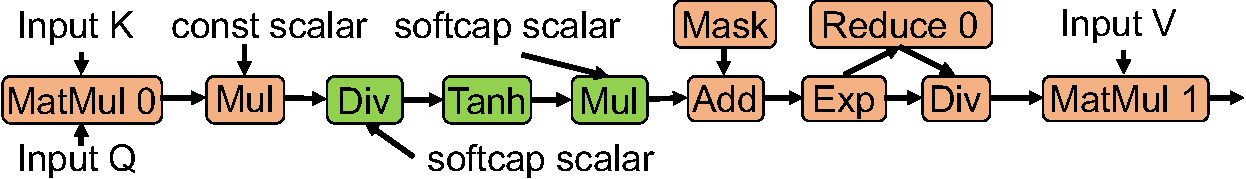
\includegraphics[width=\linewidth]{figures/flashtensor/exp_gemma2-crop.pdf}
%     \end{minipage}
%     % \vspace{-1em}
%     \\
% \centering \small (a) 标准注意力与 Gemma2 的差异。绿色算子为 Gemma2 的额外结构。  
%     \begin{minipage}[ht]{\linewidth}
%         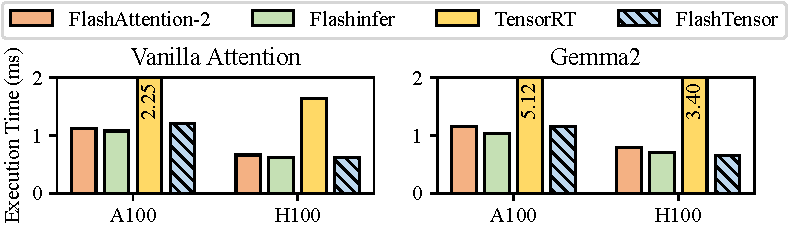
\includegraphics[width=\linewidth]{figures/flashtensor/attn_time-crop.pdf}
%     \end{minipage}
%     % \vspace{-1em}
%     \\
% \centering \small (b) 标准注意力与 Gemma2 的执行时间。截断条形图上标注了执行时间(ms)。  
%     % \vspace{-0.7em}
%     \caption{与算子库的对比}
%     % \vspace{-1.5em}
%     \label{fig:lib_cmp}
% \end{figure}  



如\Cref{fig:lib_cmp}(a) 所示,Gemma2~\cite{team2024gemma2} 在标准注意力中引入了逻辑软上限。
在\Cref{fig:lib_cmp}(b) 中,FlashTensor 与 FlashInfer 和 FlashAttention 实现了相当的性能——后两者均采用基于领域知识和人工调优的手工算子,截断条形图上标注了执行时间(ms)。
尽管 FlashTensor 未超越这些算子库,但其优势在于无需手动调优即可跨多种场景实现泛化和优化。




\subsection{性能分解分析}
本研究进行了分解分析以展示FlashTensor各个组件的性能影响,如\Cref{fig:breakdown}所示。
\begin{figure}[ht]
    \centering
    % \vspace{-1.8em}
    % \vspace{-1.6em}
    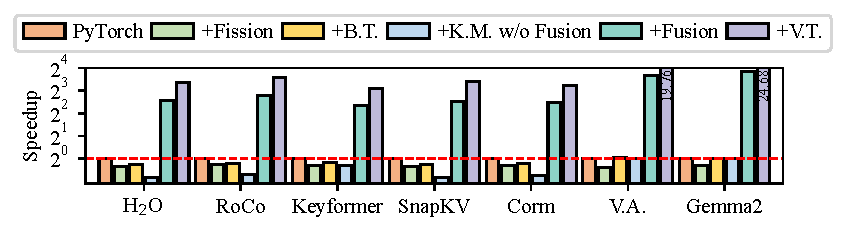
\includegraphics[width=0.85\linewidth]{figures/flashtensor/breakdown.pdf}
    % \vspace{-1.8em}
    \caption{H100上核心模块的性能分解分析}
    % \vspace{-0.5em}
    \label{fig:breakdown}
\end{figure}

基线为PyTorch,加速比为1。
FlashTensor首先应用算子裂变(Fission)将复杂算子分解为基本算子,例如将{Softmax}转换为{Exp}、{Reduce}和{Div}。
这会引入更小的算子,但增加内存访问量,从而降低整体性能。
接下来,提出基于广播属性的变换(B.T.)以最小化中间张量的大小。
这不仅提升了性能,还通过满足硬件约束为未来的融合操作创造了条件。
然后采用内核映射(K.M. w/o Fusion)来识别具有高并行效率的凸和非凸内核。
所识别的内核会重新计算一些算子以解决非凸内核的循环依赖问题,因此在未融合的情况下仍会导致性能下降。
融合操作通过减少内存访问开销并利用所识别内核的高并行效率,带来了最显著的性能提升,如\Cref{fig:breakdown}所示,加速比可达14.2倍。
最后,基于值属性的变换(V.T.)利用因果掩码消除冗余计算,在所有模型上进一步实现了近2倍的额外加速。



% \subsection{各阶段分析}
本研究进一步进行了各阶段分析,以分别展示变换和内核识别规则对性能的影响。

(1)\textbf{变换阶段}:
FlashTensor提出了一系列基于广播属性的变换规则,以最小化中间张量的大小。
如\Cref{tab:transform}所示,序列长度为4096时,中间张量的总大小显著减少了约3 GiB,这与\Cref{fig:seqlen_mem_flops}一致,实现了更低的内存使用和内存访问开销。此外,变换阶段的搜索成本非常小,约为数百毫秒。


\begin{table}[ht]
    \centering
    % \footnotesize
    \caption{基于广播变换的中间张量大小变化和执行时间}
    % \vspace{-0.5em}
    \begin{tabular}{ccc}
       \toprule
       模型  & 中间张量大小变化 & 时间(ms) \\
       \hline
       \(H_{2}O\)  & -3.30 GiB & 169.1 \\
       % \hline
       RoCo  & -3.18 GiB & 161.57 \\
       % \hline
       Keyformer  & -3.28 GiB & 223.69 \\
       % \hline
       SnapKV  & -3.30 GiB & 172.2 \\
       % \hline
       Corm  & -3.30 GiB & 166.5 \\
       % \hline
       标准注意力  & -3.98 GiB & 187.25 \\
       % \hline
       Gemma2  & -3.39 GiB & 238.25 \\
       \bottomrule
    \end{tabular}
    \label{tab:transform}
    % \vspace{-1.5em}
\end{table}




(2)\textbf{内核映射阶段}:
在确定最佳内核映射策略时,FlashTensor由于进一步引入了非凸内核定义,面临着巨大的搜索空间。
如\Cref{tab:search}所示,\#Op表示核心模块中的算子数量。\#Candidate表示剪枝后的候选数,括号内为可能的候选数。
即使算子数量较少,搜索空间仍然非常庞大。
例如,Keyformer的注意力模块仅包含24个算子,但整个搜索空间的大小达到了1.69亿。

如\Cref{tab:search}所示,Korch和TVM的调优时间很长,至少约2小时,但仍只能找到次优策略。
较长的调优时间主要来自对每个识别出的候选内核进行性能分析,需要大量时间来发现有效的调度方案。
然而,尽管FlashTensor的候选内核数量比Korch多得多,但本研究考虑了张量属性并有效剪枝了可能性能较差的候选内核,显著减少了候选集,从而能够在秒级快速选择最佳内核。

\begin{table}[ht]
    \centering
    % \footnotesize
    \caption{搜索性能}
    % \vspace{-0.5em}
    \begin{tabular}{cccccc}
    \toprule
      \multirow{2}{*}{模型} &  \multirow{2}{*}{\#Op}  & \#Candidate& \multicolumn{3}{c}{端到端搜索时间} \\
                              &  & (可能候选数)& FlashTensor & TVM & Korch \\
      \hline
      \(H_{2}O\)      & 16 & 5 (297K) & 3.03秒    & 1.8小时   & 1.6小时\\
      % \hline
      RoCo      & 19 & 7 (260万) & 8.40秒    & 2.3小时   & 3.5小时\\
      % \hline
      Keyformer & 24 & 10 (1.69亿) & 251.20秒 &3.3小时    & 失败 \\
      % \hline
      SnapKV    & 17 & 5 (20.7万) & 2.97秒    & 2.1小时   & 2.1小时\\
      % \hline
      Corm      & 17 & 5 (48万) & 4.14秒    & 失败 & 3.0小时\\
      % \hline
      V.A. & 15 & 4 (7万) & 2.42秒          & 1.5小时   & 1.4小时\\
      % \hline
      Gemma2    & 19  & 4 (170万) & 10.61秒  & 1.6小时   & 2.6小时 \\
      \bottomrule
    \end{tabular}
    \label{tab:search}
    % \vspace{-1.5em}
\end{table}


\section{结论}
本研究提出了 FlashTensor,这是一个利用细粒度张量属性优化张量程序的系统,旨在解决大模型后训练过程中,特别是长上下文任务中,因中间张量庞大而导致的内存开销大、算子计算效率低的问题。
本章首先总结了归约依赖、广播、大小和值这四个关键的张量属性,并设计了张量属性识别器,通过基于数据流的算法系统地分析计算图,准确捕获每个张量的属性。
然后,基于这些属性,本研究提出了张量属性感知优化方法,包括代数等价图变换和非凸内核映射,同时采用轻量级方案搜索方法,以找到最优的优化方案。
实验结果表明,与八种最先进的方法相比,FlashTensor 在 H100 上的端到端性能和核心模块性能平均加速比分别达到 1.50 倍和 3.24 倍,在 A100 上分别为 1.86 倍和 3.70 倍。

% 未来,本研究计划进一步扩展 FlashTensor 的应用范围,将其应用于更多类型的 DNN 模型和任务中。同时,我们将探索如何更好地结合硬件特性,进一步优化张量属性感知的优化策略,以实现更高的计算效率和更低的资源消耗。此外,我们还将研究如何将 FlashTensor 与其他深度学习优化技术相结合,形成更强大的优化框架,推动深度学习在更多领域的应用和发展。
